% Options for packages loaded elsewhere
\PassOptionsToPackage{unicode}{hyperref}
\PassOptionsToPackage{hyphens}{url}
%
\documentclass[
]{article}
\usepackage{amsmath,amssymb}
\usepackage{iftex}
\ifPDFTeX
  \usepackage[T1]{fontenc}
  \usepackage[utf8]{inputenc}
  \usepackage{textcomp} % provide euro and other symbols
\else % if luatex or xetex
  \usepackage{unicode-math} % this also loads fontspec
  \defaultfontfeatures{Scale=MatchLowercase}
  \defaultfontfeatures[\rmfamily]{Ligatures=TeX,Scale=1}
\fi
\usepackage{lmodern}
\ifPDFTeX\else
  % xetex/luatex font selection
\fi
% Use upquote if available, for straight quotes in verbatim environments
\IfFileExists{upquote.sty}{\usepackage{upquote}}{}
\IfFileExists{microtype.sty}{% use microtype if available
  \usepackage[]{microtype}
  \UseMicrotypeSet[protrusion]{basicmath} % disable protrusion for tt fonts
}{}
\makeatletter
\@ifundefined{KOMAClassName}{% if non-KOMA class
  \IfFileExists{parskip.sty}{%
    \usepackage{parskip}
  }{% else
    \setlength{\parindent}{0pt}
    \setlength{\parskip}{6pt plus 2pt minus 1pt}}
}{% if KOMA class
  \KOMAoptions{parskip=half}}
\makeatother
\usepackage{xcolor}
\usepackage[margin=1in]{geometry}
\usepackage{color}
\usepackage{fancyvrb}
\newcommand{\VerbBar}{|}
\newcommand{\VERB}{\Verb[commandchars=\\\{\}]}
\DefineVerbatimEnvironment{Highlighting}{Verbatim}{commandchars=\\\{\}}
% Add ',fontsize=\small' for more characters per line
\usepackage{framed}
\definecolor{shadecolor}{RGB}{248,248,248}
\newenvironment{Shaded}{\begin{snugshade}}{\end{snugshade}}
\newcommand{\AlertTok}[1]{\textcolor[rgb]{0.94,0.16,0.16}{#1}}
\newcommand{\AnnotationTok}[1]{\textcolor[rgb]{0.56,0.35,0.01}{\textbf{\textit{#1}}}}
\newcommand{\AttributeTok}[1]{\textcolor[rgb]{0.13,0.29,0.53}{#1}}
\newcommand{\BaseNTok}[1]{\textcolor[rgb]{0.00,0.00,0.81}{#1}}
\newcommand{\BuiltInTok}[1]{#1}
\newcommand{\CharTok}[1]{\textcolor[rgb]{0.31,0.60,0.02}{#1}}
\newcommand{\CommentTok}[1]{\textcolor[rgb]{0.56,0.35,0.01}{\textit{#1}}}
\newcommand{\CommentVarTok}[1]{\textcolor[rgb]{0.56,0.35,0.01}{\textbf{\textit{#1}}}}
\newcommand{\ConstantTok}[1]{\textcolor[rgb]{0.56,0.35,0.01}{#1}}
\newcommand{\ControlFlowTok}[1]{\textcolor[rgb]{0.13,0.29,0.53}{\textbf{#1}}}
\newcommand{\DataTypeTok}[1]{\textcolor[rgb]{0.13,0.29,0.53}{#1}}
\newcommand{\DecValTok}[1]{\textcolor[rgb]{0.00,0.00,0.81}{#1}}
\newcommand{\DocumentationTok}[1]{\textcolor[rgb]{0.56,0.35,0.01}{\textbf{\textit{#1}}}}
\newcommand{\ErrorTok}[1]{\textcolor[rgb]{0.64,0.00,0.00}{\textbf{#1}}}
\newcommand{\ExtensionTok}[1]{#1}
\newcommand{\FloatTok}[1]{\textcolor[rgb]{0.00,0.00,0.81}{#1}}
\newcommand{\FunctionTok}[1]{\textcolor[rgb]{0.13,0.29,0.53}{\textbf{#1}}}
\newcommand{\ImportTok}[1]{#1}
\newcommand{\InformationTok}[1]{\textcolor[rgb]{0.56,0.35,0.01}{\textbf{\textit{#1}}}}
\newcommand{\KeywordTok}[1]{\textcolor[rgb]{0.13,0.29,0.53}{\textbf{#1}}}
\newcommand{\NormalTok}[1]{#1}
\newcommand{\OperatorTok}[1]{\textcolor[rgb]{0.81,0.36,0.00}{\textbf{#1}}}
\newcommand{\OtherTok}[1]{\textcolor[rgb]{0.56,0.35,0.01}{#1}}
\newcommand{\PreprocessorTok}[1]{\textcolor[rgb]{0.56,0.35,0.01}{\textit{#1}}}
\newcommand{\RegionMarkerTok}[1]{#1}
\newcommand{\SpecialCharTok}[1]{\textcolor[rgb]{0.81,0.36,0.00}{\textbf{#1}}}
\newcommand{\SpecialStringTok}[1]{\textcolor[rgb]{0.31,0.60,0.02}{#1}}
\newcommand{\StringTok}[1]{\textcolor[rgb]{0.31,0.60,0.02}{#1}}
\newcommand{\VariableTok}[1]{\textcolor[rgb]{0.00,0.00,0.00}{#1}}
\newcommand{\VerbatimStringTok}[1]{\textcolor[rgb]{0.31,0.60,0.02}{#1}}
\newcommand{\WarningTok}[1]{\textcolor[rgb]{0.56,0.35,0.01}{\textbf{\textit{#1}}}}
\usepackage{graphicx}
\makeatletter
\def\maxwidth{\ifdim\Gin@nat@width>\linewidth\linewidth\else\Gin@nat@width\fi}
\def\maxheight{\ifdim\Gin@nat@height>\textheight\textheight\else\Gin@nat@height\fi}
\makeatother
% Scale images if necessary, so that they will not overflow the page
% margins by default, and it is still possible to overwrite the defaults
% using explicit options in \includegraphics[width, height, ...]{}
\setkeys{Gin}{width=\maxwidth,height=\maxheight,keepaspectratio}
% Set default figure placement to htbp
\makeatletter
\def\fps@figure{htbp}
\makeatother
\setlength{\emergencystretch}{3em} % prevent overfull lines
\providecommand{\tightlist}{%
  \setlength{\itemsep}{0pt}\setlength{\parskip}{0pt}}
\setcounter{secnumdepth}{-\maxdimen} % remove section numbering
\usepackage{booktabs}
\usepackage{longtable}
\usepackage{array}
\usepackage{multirow}
\usepackage{wrapfig}
\usepackage{float}
\usepackage{colortbl}
\usepackage{pdflscape}
\usepackage{tabu}
\usepackage{threeparttable}
\usepackage{threeparttablex}
\usepackage[normalem]{ulem}
\usepackage{makecell}
\usepackage{xcolor}
\ifLuaTeX
  \usepackage{selnolig}  % disable illegal ligatures
\fi
\IfFileExists{bookmark.sty}{\usepackage{bookmark}}{\usepackage{hyperref}}
\IfFileExists{xurl.sty}{\usepackage{xurl}}{} % add URL line breaks if available
\urlstyle{same}
\hypersetup{
  pdftitle={HW3},
  pdfauthor={Zirui Zhang},
  hidelinks,
  pdfcreator={LaTeX via pandoc}}

\title{HW3}
\author{Zirui Zhang}
\date{2023-09-30}

\begin{document}
\maketitle

\hypertarget{question-3}{%
\section{Question 3}\label{question-3}}

\begin{Shaded}
\begin{Highlighting}[]
\NormalTok{data }\OtherTok{=}\NormalTok{ ovarian }\SpecialCharTok{\%\textgreater{}\%} \FunctionTok{mutate}\NormalTok{(}\AttributeTok{fustat =} \FunctionTok{as.factor}\NormalTok{(fustat), }\AttributeTok{rx =} \FunctionTok{as.factor}\NormalTok{(rx))}
\NormalTok{ovarian.survfit }\OtherTok{=}\NormalTok{ ovarian }\SpecialCharTok{\%\textgreater{}\%} \FunctionTok{survfit}\NormalTok{(}\FunctionTok{Surv}\NormalTok{(futime, fustat) }\SpecialCharTok{\textasciitilde{}}\NormalTok{ rx, }\AttributeTok{data =}\NormalTok{ .)}
\NormalTok{ovarian.survfit }\SpecialCharTok{\%\textgreater{}\%} \FunctionTok{autoplot}\NormalTok{() }\SpecialCharTok{+} \FunctionTok{ylab}\NormalTok{(}\StringTok{"S(t)"}\NormalTok{) }\SpecialCharTok{+} \FunctionTok{xlab}\NormalTok{(}\StringTok{"Time"}\NormalTok{)}
\end{Highlighting}
\end{Shaded}

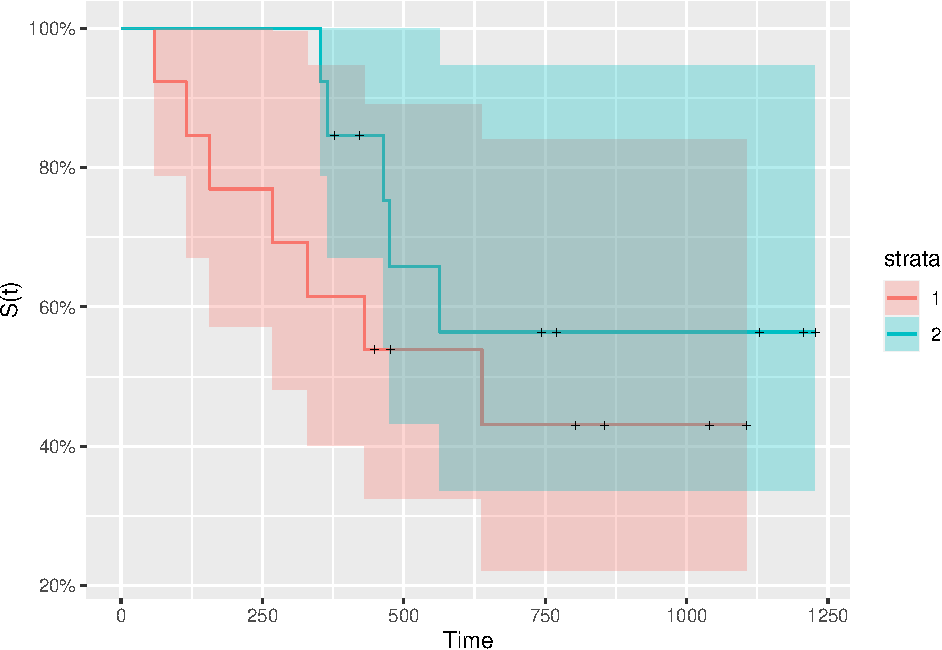
\includegraphics{HW3_files/figure-latex/unnamed-chunk-1-1.pdf}

\hypertarget{create-life-time-stratified-by-rx}{%
\subsubsection{1. Create life-time stratified by
rx}\label{create-life-time-stratified-by-rx}}

\begin{Shaded}
\begin{Highlighting}[]
\CommentTok{\# Create life{-}table stratified by rx}
\NormalTok{lt1 }\OtherTok{=} \FunctionTok{lifetab2}\NormalTok{(}\FunctionTok{Surv}\NormalTok{(futime, fustat }\SpecialCharTok{==} \DecValTok{1}\NormalTok{) }\SpecialCharTok{\textasciitilde{}} \DecValTok{1}\NormalTok{, }
\NormalTok{               data[data}\SpecialCharTok{$}\NormalTok{rx }\SpecialCharTok{==} \DecValTok{1}\NormalTok{, ], }
               \AttributeTok{breaks=} \FunctionTok{seq}\NormalTok{(}\DecValTok{0}\NormalTok{, }\DecValTok{1300}\NormalTok{, }\DecValTok{100}\NormalTok{)) }\CommentTok{\#rx=1}
\NormalTok{lt2 }\OtherTok{=} \FunctionTok{lifetab2}\NormalTok{(}\FunctionTok{Surv}\NormalTok{(futime, fustat }\SpecialCharTok{==} \DecValTok{1}\NormalTok{) }\SpecialCharTok{\textasciitilde{}} \DecValTok{1}\NormalTok{, }
\NormalTok{               data[data}\SpecialCharTok{$}\NormalTok{rx }\SpecialCharTok{==} \DecValTok{2}\NormalTok{, ], }
               \AttributeTok{breaks=} \FunctionTok{seq}\NormalTok{(}\DecValTok{0}\NormalTok{, }\DecValTok{1300}\NormalTok{, }\DecValTok{100}\NormalTok{)) }\CommentTok{\#rx=2}
\FunctionTok{options}\NormalTok{(}\AttributeTok{digits=}\DecValTok{2}\NormalTok{)}
\NormalTok{lt1 }\SpecialCharTok{\%\textgreater{}\%} \FunctionTok{kable}\NormalTok{(}\AttributeTok{caption =} \StringTok{"Life{-}table for treatment 1"}\NormalTok{) }\CommentTok{\# life{-}table for treatment 1}
\end{Highlighting}
\end{Shaded}

\begin{table}

\caption{\label{tab:unnamed-chunk-2}Life-table for treatment 1}
\centering
\begin{tabular}[t]{l|r|r|r|r|r|r|r|r|r|r|r|r}
\hline
  & tstart & tstop & nsubs & nlost & nrisk & nevent & surv & pdf & hazard & se.surv & se.pdf & se.hazard\\
\hline
0-100 & 0 & 100 & 13 & 0 & 13.0 & 1 & 1.00 & 0 & 0 & 0.00 & 0 & 0\\
\hline
100-200 & 100 & 200 & 12 & 0 & 12.0 & 2 & 0.92 & 0 & 0 & 0.07 & 0 & 0\\
\hline
200-300 & 200 & 300 & 10 & 0 & 10.0 & 1 & 0.77 & 0 & 0 & 0.12 & 0 & 0\\
\hline
300-400 & 300 & 400 & 9 & 0 & 9.0 & 1 & 0.69 & 0 & 0 & 0.13 & 0 & 0\\
\hline
400-500 & 400 & 500 & 8 & 2 & 7.0 & 1 & 0.62 & 0 & 0 & 0.13 & 0 & 0\\
\hline
500-600 & 500 & 600 & 5 & 0 & 5.0 & 0 & 0.53 & 0 & 0 & 0.14 & NaN & NaN\\
\hline
600-700 & 600 & 700 & 5 & 0 & 5.0 & 1 & 0.53 & 0 & 0 & 0.14 & 0 & 0\\
\hline
700-800 & 700 & 800 & 4 & 0 & 4.0 & 0 & 0.42 & 0 & 0 & 0.15 & NaN & NaN\\
\hline
800-900 & 800 & 900 & 4 & 2 & 3.0 & 0 & 0.42 & 0 & 0 & 0.15 & NaN & NaN\\
\hline
900-1000 & 900 & 1000 & 2 & 0 & 2.0 & 0 & 0.42 & 0 & 0 & 0.15 & NaN & NaN\\
\hline
1000-1100 & 1000 & 1100 & 2 & 1 & 1.5 & 0 & 0.42 & 0 & 0 & 0.15 & NaN & NaN\\
\hline
1100-1200 & 1100 & 1200 & 1 & 1 & 0.5 & 0 & 0.42 & 0 & 0 & 0.15 & NaN & NaN\\
\hline
1200-1300 & 1200 & 1300 & 0 & 0 & 0.0 & 0 & 0.42 & NaN & NaN & 0.15 & NaN & NaN\\
\hline
1300-Inf & 1300 & Inf & 0 & 0 & 0.0 & 0 & NaN & NA & NA & NaN & NA & NA\\
\hline
\end{tabular}
\end{table}

\begin{Shaded}
\begin{Highlighting}[]
\NormalTok{lt2 }\SpecialCharTok{\%\textgreater{}\%} \FunctionTok{kable}\NormalTok{(}\AttributeTok{caption =} \StringTok{"Life{-}table for treatment 2"}\NormalTok{) }\CommentTok{\# life{-}table for treatment 2}
\end{Highlighting}
\end{Shaded}

\begin{table}

\caption{\label{tab:unnamed-chunk-2}Life-table for treatment 2}
\centering
\begin{tabular}[t]{l|r|r|r|r|r|r|r|r|r|r|r|r}
\hline
  & tstart & tstop & nsubs & nlost & nrisk & nevent & surv & pdf & hazard & se.surv & se.pdf & se.hazard\\
\hline
0-100 & 0 & 100 & 13 & 0 & 13.0 & 0 & 1.00 & 0 & 0 & 0.00 & NaN & NaN\\
\hline
100-200 & 100 & 200 & 13 & 0 & 13.0 & 0 & 1.00 & 0 & 0 & 0.00 & NaN & NaN\\
\hline
200-300 & 200 & 300 & 13 & 0 & 13.0 & 0 & 1.00 & 0 & 0 & 0.00 & NaN & NaN\\
\hline
300-400 & 300 & 400 & 13 & 1 & 12.5 & 2 & 1.00 & 0 & 0 & 0.00 & 0 & 0\\
\hline
400-500 & 400 & 500 & 10 & 1 & 9.5 & 2 & 0.84 & 0 & 0 & 0.10 & 0 & 0\\
\hline
500-600 & 500 & 600 & 7 & 0 & 7.0 & 1 & 0.66 & 0 & 0 & 0.14 & 0 & 0\\
\hline
600-700 & 600 & 700 & 6 & 0 & 6.0 & 0 & 0.57 & 0 & 0 & 0.15 & NaN & NaN\\
\hline
700-800 & 700 & 800 & 6 & 3 & 4.5 & 0 & 0.57 & 0 & 0 & 0.15 & NaN & NaN\\
\hline
800-900 & 800 & 900 & 3 & 0 & 3.0 & 0 & 0.57 & 0 & 0 & 0.15 & NaN & NaN\\
\hline
900-1000 & 900 & 1000 & 3 & 0 & 3.0 & 0 & 0.57 & 0 & 0 & 0.15 & NaN & NaN\\
\hline
1000-1100 & 1000 & 1100 & 3 & 0 & 3.0 & 0 & 0.57 & 0 & 0 & 0.15 & NaN & NaN\\
\hline
1100-1200 & 1100 & 1200 & 3 & 1 & 2.5 & 0 & 0.57 & 0 & 0 & 0.15 & NaN & NaN\\
\hline
1200-1300 & 1200 & 1300 & 2 & 2 & 1.0 & 0 & 0.57 & 0 & 0 & 0.15 & NaN & NaN\\
\hline
1300-Inf & 1300 & Inf & 0 & 0 & 0.0 & 0 & 0.57 & NA & NA & 0.15 & NA & NA\\
\hline
\end{tabular}
\end{table}

\hypertarget{plot-harzard-function-by-rx}{%
\subsubsection{2. Plot harzard function by
rx}\label{plot-harzard-function-by-rx}}

\begin{Shaded}
\begin{Highlighting}[]
\FunctionTok{ggplot}\NormalTok{(lt1, }\FunctionTok{aes}\NormalTok{(}\AttributeTok{x =}\NormalTok{ tstart, }\AttributeTok{xend =}\NormalTok{ tstop, }\AttributeTok{y =}\NormalTok{ hazard, }\AttributeTok{yend =}\NormalTok{ hazard)) }\SpecialCharTok{+}
  \FunctionTok{geom\_segment}\NormalTok{() }\SpecialCharTok{+}
  \FunctionTok{labs}\NormalTok{(}\AttributeTok{x =} \StringTok{"t"}\NormalTok{, }\AttributeTok{y =} \StringTok{"h(t)"}\NormalTok{) }\SpecialCharTok{+}
  \FunctionTok{ggtitle}\NormalTok{(}\StringTok{"Hazard function for treatment 1"}\NormalTok{) }\SpecialCharTok{+}
  \FunctionTok{theme\_minimal}\NormalTok{() }\CommentTok{\#rx=1}
\end{Highlighting}
\end{Shaded}

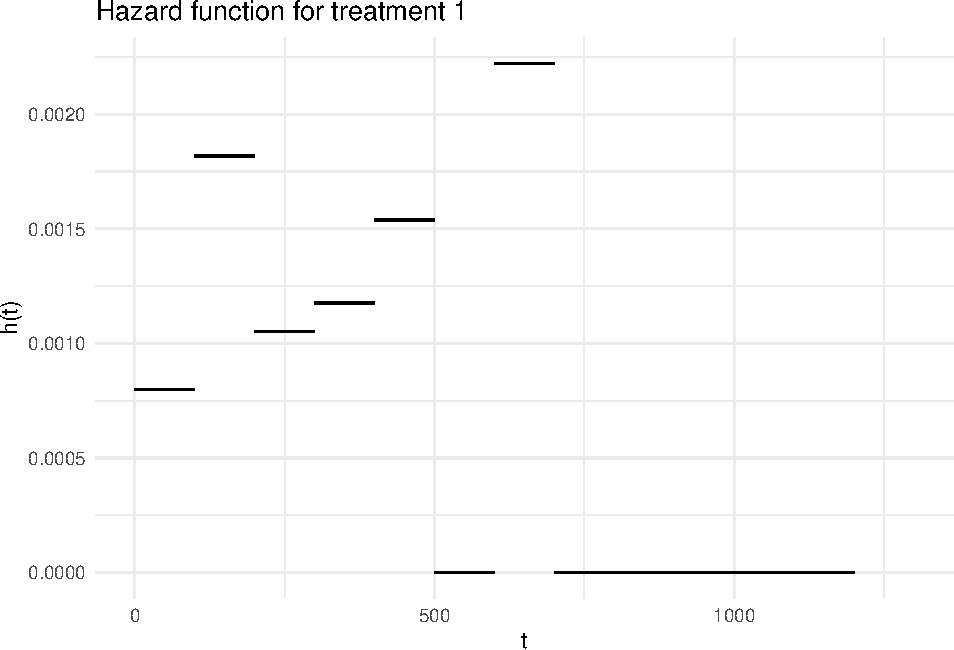
\includegraphics{HW3_files/figure-latex/unnamed-chunk-3-1.pdf}

\begin{Shaded}
\begin{Highlighting}[]
\FunctionTok{ggplot}\NormalTok{(lt2, }\FunctionTok{aes}\NormalTok{(}\AttributeTok{x =}\NormalTok{ tstart, }\AttributeTok{xend =}\NormalTok{ tstop, }\AttributeTok{y =}\NormalTok{ hazard, }\AttributeTok{yend =}\NormalTok{ hazard)) }\SpecialCharTok{+}
  \FunctionTok{geom\_segment}\NormalTok{() }\SpecialCharTok{+}
  \FunctionTok{labs}\NormalTok{(}\AttributeTok{x =} \StringTok{"t"}\NormalTok{, }\AttributeTok{y =} \StringTok{"h(t)"}\NormalTok{) }\SpecialCharTok{+}
  \FunctionTok{ggtitle}\NormalTok{(}\StringTok{"Hazard function for treatment 2"}\NormalTok{)}\SpecialCharTok{+}
  \FunctionTok{theme\_minimal}\NormalTok{() }\CommentTok{\#rx=2}
\end{Highlighting}
\end{Shaded}

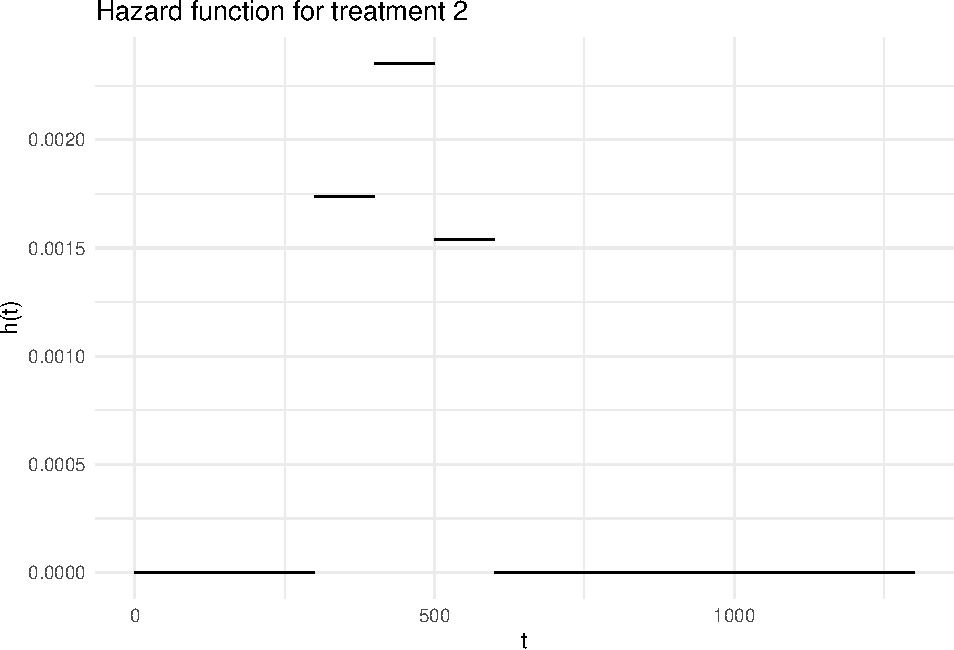
\includegraphics{HW3_files/figure-latex/unnamed-chunk-3-2.pdf}

\hypertarget{plot-k-m-survival-function-by-rx}{%
\subsubsection{3. Plot K-M survival function by
rx}\label{plot-k-m-survival-function-by-rx}}

\begin{Shaded}
\begin{Highlighting}[]
\NormalTok{mfit }\OtherTok{=} \FunctionTok{survfit}\NormalTok{(}\FunctionTok{Surv}\NormalTok{(futime, fustat }\SpecialCharTok{==} \DecValTok{1}\NormalTok{) }\SpecialCharTok{\textasciitilde{}}\NormalTok{ rx, data)}
\FunctionTok{plot}\NormalTok{(mfit, }\AttributeTok{ylab=}\StringTok{"S(t)"}\NormalTok{, }\AttributeTok{xlab=}\StringTok{"Time in days"}\NormalTok{,}
     \AttributeTok{main =} \StringTok{"Kaplan−Meier estimates of treatment{-}specific survival"}\NormalTok{)}
\end{Highlighting}
\end{Shaded}

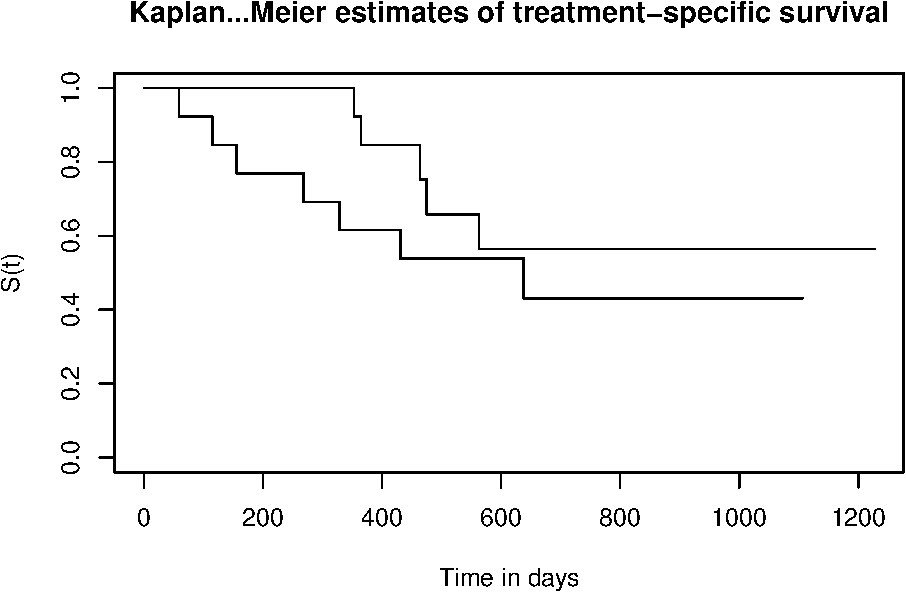
\includegraphics{HW3_files/figure-latex/unnamed-chunk-4-1.pdf}

\hypertarget{median-for-each-treatment-group}{%
\subsubsection{4. Median for each treatment
group}\label{median-for-each-treatment-group}}

\begin{itemize}
\tightlist
\item
  rx 1: median = 638
\item
  rx 2: median doesn't exist
\end{itemize}

\begin{Shaded}
\begin{Highlighting}[]
\FunctionTok{print}\NormalTok{(mfit)}
\end{Highlighting}
\end{Shaded}

\begin{verbatim}
## Call: survfit(formula = Surv(futime, fustat == 1) ~ rx, data = data)
## 
##       n events median 0.95LCL 0.95UCL
## rx=1 13      7    638     268      NA
## rx=2 13      5     NA     475      NA
\end{verbatim}

\hypertarget{compare-survival-function-estimations-between-k-m-and-f-h-methods}{%
\subsubsection{5. Compare survival function estimations between K-M and
F-H
methods}\label{compare-survival-function-estimations-between-k-m-and-f-h-methods}}

\begin{Shaded}
\begin{Highlighting}[]
\NormalTok{hfit }\OtherTok{=} \FunctionTok{survfit}\NormalTok{(}\FunctionTok{Surv}\NormalTok{(futime, fustat }\SpecialCharTok{==} \DecValTok{1}\NormalTok{) }\SpecialCharTok{\textasciitilde{}}\NormalTok{ rx, }\AttributeTok{type =} \StringTok{"fleming{-}harrington"}\NormalTok{, data)}
\FunctionTok{summary}\NormalTok{(hfit)}
\end{Highlighting}
\end{Shaded}

\begin{verbatim}
## Call: survfit(formula = Surv(futime, fustat == 1) ~ rx, data = data, 
##     type = "fleming-harrington")
## 
##                 rx=1 
##  time n.risk n.event survival std.err lower 95% CI upper 95% CI
##    59     13       1    0.926  0.0712        0.796        1.000
##   115     12       1    0.852  0.0966        0.682        1.000
##   156     11       1    0.778  0.1131        0.585        1.000
##   268     10       1    0.704  0.1242        0.498        0.995
##   329      9       1    0.630  0.1313        0.419        0.948
##   431      8       1    0.556  0.1351        0.345        0.895
##   638      5       1    0.455  0.1433        0.246        0.843
## 
##                 rx=2 
##  time n.risk n.event survival std.err lower 95% CI upper 95% CI
##   353     13       1    0.926  0.0712        0.796        1.000
##   365     12       1    0.852  0.0966        0.682        1.000
##   464      9       1    0.762  0.1210        0.558        1.000
##   475      8       1    0.673  0.1359        0.453        1.000
##   563      7       1    0.583  0.1443        0.359        0.947
\end{verbatim}

\begin{Shaded}
\begin{Highlighting}[]
\FunctionTok{print}\NormalTok{(hfit)}
\end{Highlighting}
\end{Shaded}

\begin{verbatim}
## Call: survfit(formula = Surv(futime, fustat == 1) ~ rx, data = data, 
##     type = "fleming-harrington")
## 
##       n events median 0.95LCL 0.95UCL
## rx=1 13      7    638     268      NA
## rx=2 13      5     NA     475      NA
\end{verbatim}

\end{document}
